\documentclass{article}



%% For IPA  
\usepackage{tipa}


%% for xeCJK
\usepackage{xeCJK}
\setCJKmainfont{SimSun}

\usepackage{xcolor}
\usepackage{hyperref}

\usepackage{amsmath}
\usepackage{pgf}
\usepackage{tikz}
\usetikzlibrary{arrows,shapes,snakes,automata,backgrounds,petri,matrix,arrows,arrows,%
    decorations.pathmorphing,decorations,backgrounds,decorations.text,%
    decorations.fractals,shadows,patterns,fadings,shapes,through,fit,positioning,scopes%
    }

%% subfigure
\usepackage{subfigure}

%% title and author
\title{The Analysis of Hpeg}
\author{李约瀚 \\ 14130140331 \\ me@qinka.pro \\ qinka@live.com}

\begin{document}

%% title and table of content
\maketitle
\newpage
\tableofcontents
\newpage

%% Summary
\section{Summary}
\label{sec:summary}

This report is about Hpeg. The workflow of the Hpeg's encoding and decoding processes will be talked about, firstly. And next one is the structure of the codes. Finally, the influence of the noise, and test will be discussed.

In the worst case, the ratio of compression is about 30\% to 40\%,
and in the best case, the ratio of compression is about 1\% to 10\%.
The influence of the noise mainly caused by the errors in the DCT; by using more bits to store the 
information, the errors can reduce.

%% Hpeg
\section{Hpeg}
\label{sec:hpeg}

\subsection{About}
\label{sec:hpeg:about}

Hpeg(\textipa{/"eItS""pEg/}) is another jpeg-like method of compression for digital images, written by me.
Hpeg is using DCT(Discrete Cosine Transform) as lossy compression method, and spare matrix as the entropy coding method.
Meanwhile, the final datas are compressed with lzma compression algorithm for using spare matrix to code. 

The project Hpeg's codes had been already opened on \href{http://github.com/Qinka/hpeg.hs}{GitHub}.
Until now, however, there is not any document for this project but just some comment in Haddock.
Hpeg is written in Haskell, and its algorithms are design for running on the GPU with many computing unit.
That program can run with a GPU which supports CUDA,and it use library \href{https://github.com/AccelerateHS/accelerate}{accelerate}.
But unfortunately, building this program might be an ugly thing.

The program take a Window BMP image as input and will output the .hpeg file,
and it also take a .hpeg as input and output a Window BMP image with RGBA\footnote{For A in the RGBA, is constant 0xFF}.

\subsection{Inside}
\label{sec:hpeg:inside}

Hpeg is using DCT and spare matrix, and now let's talk about the general workflow of encoding to Hpeg. The first thing to do is reading from the .bmp file.
Next, the colors under RGB need to be convert to YCbCr, because when using DCT the color space YCbCr will be used. 
Then the luminance and chroma will be transformed by DCT. Then the transformed matrix will be encoded with spare matrix.
Finally, the encoded one will be stored on the disk. However the data will be compressed with LZMA before it's stored.

So the decoding is similar with encoding. The first thing to do is reading from file, and constructing from spare matrix.
Next, matrix transform with IDCT(Inverse Discrete Cosine Transform). After the colors under YCbCr got, the colors will be convert
back to RGB. Finally, the datas will be written into a .bmp file. The figure \ref{fig:hpeg:workflow} might be more visual.

\begin{figure}
    \centering
    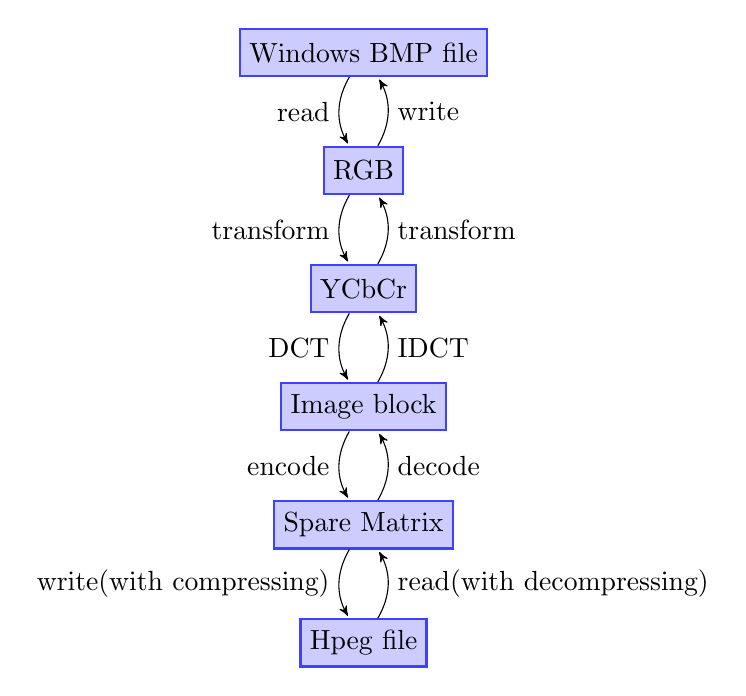
\begin{tikzpicture}[node distance=1.5cm,>=stealth',bend angle=30,auto]
        \tikzstyle{point}=[rectangle,thick,draw=blue!75,fill=blue!20,minimum size=6mm]
        \begin{scope}
        \node[point](bmp){Windows BMP file};
        \node[point](rgb)[below of=bmp]{RGB}
            edge [pre,bend left]   node         {read} (bmp)
            edge [post,bend right] node [right] {write}(bmp);
        \node[point](ycbcr)[below of=rgb]{YCbCr}
            edge [pre,bend left]   node         {transform}(rgb)
            edge [post,bend right] node [right] {transform}(rgb);
        \node[point](ib)[below of=ycbcr]{Image block}
            edge [pre,bend left]   node         {DCT}(ycbcr)
            edge [post,bend right] node [right] {IDCT}(ycbcr);
        \node[point](sm)[below of=ib]{Spare Matrix}
            edge [pre,bend left]   node         {encode}(ib)
            edge [post,bend right] node [right] {decode}(ib);
        \node[point](hpeg)[below of=sm]{Hpeg file}
            edge [pre,bend left]   node         {write(with compressing)}(sm)
            edge [post,bend right] node [right] {read(with decompressing)}(sm);
        \end{scope}
    \end{tikzpicture}
    \caption{Workflow of Hpeg Encoding and Decoding}
    \label{fig:hpeg:workflow}
\end{figure}

\subsubsection{Convertion for Color Space}
\label{sec:hpeg:inside:cfcs}

The first task in encoding and decoding is converting between two color spaces: RGB, and YCbCr.
The Eq.\ref{eq:colorspaceconvert1} and Eq.\ref{eq:colorspaceconvert2} are the equations for converting
between RGB and YCbCr, where $R,G,B \in \left[0,255\right]$ mean ``red'', ``blue'', and ``green'',
and $Y \in \left[-15,15\right]$ and $Cb,Cr \in \left[-127,127\right]$ mean ``luminance'', blue-diff chroma component, and red-diff chroma component.
\begin{equation}
    \label{eq:colorspaceconvert1}
    \left\{\begin{array}{rcl}
    Y  &=& 0.257R+0.564G+0.098B+16 \\
    Cb &=& -0.147R-0.291G+0.439B+128 \\
    Cr &=& 0.439R-0.368G-0.071B+128
    \end{array}\right.
\end{equation}
\begin{equation}
    \label{eq:colorspaceconvert2}
    \left\{\begin{array}{rcl}
    R &=& 1.164(Y-16) + 1.596(Cr-128) \\
    G &=& 1.164(Y-16) - 0.392(Cb-128)-0.813(Cr-128) \\
    B &=& 1.164(Y-16) + 2.017(Cb-128)
    \end{array}\right.
\end{equation}

So with Eq.\ref{eq:colorspaceconvert1} and Eq.\ref{eq:colorspaceconvert2},
the matrices of color will be convert between RGB and YCbCr in GPU.

\subsubsection{DCT \& IDCT}
\label{sec:hpeg:inside:dct}

After the colors converted to YCbCr color space, the matrices of the color need to be transformed with DCT.
Meanwhile, before the colors converted to RGB in decoding, the matrices of the color need to be transformed
with IDCT.

For 2D Discrete Cosine Transformation, its equation is Eq.\ref{eq:dct2}.
\begin{equation}
\label{eq:dct2}
F(u,v) = \frac{2C(u)C(v)}{\sqrt{MN}}\sum\limits_{i=0}^{M-1}\sum\limits_{j=0}^{N-1}\cos{\frac{(2i+1)u\pi}{2M}}\cos{\frac{(2j+1)v\pi}{2N}}f(i,j)
\end{equation}
where $i,u=0,1,\cdots,M-1$,$j,v=0,1,...,N-1$, and the constants $C(u)$ and $C(v)$ are determined by
\begin{equation}
\label{eq:2dct}
C(\xi) = \left\{
\begin{array}{cc}
\frac{\sqrt{2}}{2} & \xi = 0, \\
1 & otherwise.
\end{array}\right.
\end{equation}
Meanwhile the Eq.\ref{eq:idct2} is the 2D Inverse Discrete Cosine Transform.
\begin{equation}
\label{eq:idct2}
\widetilde{f}(i,j) = \sum\limits_{u=0}^{M-1}\sum\limits_{v=0}^{N-1}\frac{2C(u)C(v)}{\sqrt{MN}}\cos{\frac{(2i+1)u\pi}{2M}}\cos{\frac{(2j+1)v\pi}{2N}}F(i,j)
\end{equation} 

For both DCT and IDCT, the baisc unit is a $8 \times 8$ block, and each block is independent with other block.

\subsubsection{Spare Matrix}
\label{sec:hpeg:inside:sparematrix}

In the each block, the matrix transformed with DCT need to be quantized and encoding, when encoding.
It is similar in decoding. And the tables for quantization are table \ref{tab:luminacequantization} and
table \ref{tab:chromonacequantization}.

\begin{table}
    \centering
    \caption{The luminance quantization table.}
    \begin{tabular}{rrrrrrrr}
        \hline
        16 & 11 & 10 & 16 & 24 & 40 & 51 & 61 \\ 
        12 & 12 & 14 & 19 & 26 & 58 & 60 & 55 \\ 
        14 & 13 & 16 & 24 & 40 & 57 & 69 & 56 \\ 
        14 & 17 & 22 & 29 & 51 & 87 & 80 & 62 \\ 
        18 & 22 & 37 & 56 & 68 & 109 & 103 & 77 \\ 
        24 & 35 & 55 & 64 & 81 & 104 & 113 & 92 \\ 
        49 & 64 & 78 & 87 & 103 & 121 & 120 & 101 \\ 
        72 & 92 & 95 & 98 & 112 & 100 & 103 & 99 \\
        \hline
    \end{tabular}
    \label{tab:luminacequantization}
\end{table}

\begin{table}
    \centering
    \caption{The chromonace quantization table.}
    \begin{tabular}{rrrrrrrr}
        \hline
        17 & 18 & 24 & 47 & 99 & 99 & 99 & 99 \\ 
        18 & 21 & 26 & 66 & 99 & 99 & 99 & 99 \\ 
        24 & 26 & 56 & 99 & 99 & 99 & 99 & 99 \\ 
        47 & 66 & 99 & 99 & 99 & 99 & 99 & 99 \\ 
        99 & 99 & 99 & 99 & 99 & 99 & 99 & 99 \\ 
        99 & 99 & 99 & 99 & 99 & 99 & 99 & 99 \\ 
        99 & 99 & 99 & 99 & 99 & 99 & 99 & 99 \\ 
        99 & 99 & 99 & 99 & 99 & 99 & 99 & 99 \\
        \hline
    \end{tabular} 
    \label{tab:chromonacequantization}
\end{table}

The operation of the quantization is:
\begin{equation}
\label{eq:quantization}
\widehat{F}(u,v) = round\left(\frac{F(u,v)}{Q(u,v)}\right)
\end{equation}
where $F(u,v)$ is the transformed matrix, and $Q(u,v)$ is the matrix of the quantization.

For decoding, Eq.\ref{eq:quantization} will not work, and the following is needed:
\begin{equation}
\label{eq:iquantization}
F(u,v) = \left(\widehat{F}(u,v) \times Q(u,v)\right)
\end{equation}

After quantizing, the matrix will be represent with spare matrix.
The elements in the representation are index and the value. The higher 4-bit of the index is for ``u'',
and the lower 4-bit of the index is for ``v'', where $u$ and $v$ are the one in the Eq.\ref{eq:dct2}.
Both of the higher part and lower part's highest bit is reserved, for $u,v \in \left[0,7\right]$.

An item, a tuple of index and value, holds a non-zero element in the matrix.
And a list or array of the items represent a $8 \times 8$ matrix.
Then a list of array of the matrices represent a image or just say colors.

\subsubsection{Store}
\label{sec:hpeg:inside:store}

So till now, a Hpeg image includes the height, weight, Y's matrices, Cb's matrices, and Cr's matrices.
Meanwhile, Hpeg file also has a magic number at the beginning of the file -- "HpEg" in ASCII.

All this things will be serialized to or deserialized from bytes, as well as them will be written to or
read from the file.

\subsection{Codes}
\label{sec:hpeg:codes}

The codes of Hpeg has 5 modules. And they are organized as what figure \ref{fig:hpeg:layout} showed.

\begin{figure}
    \centering
    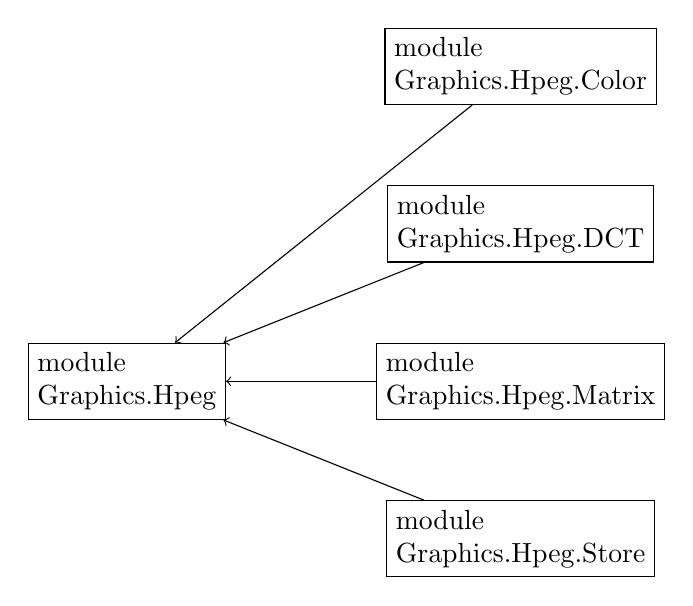
\begin{tikzpicture}[baseline=-.3em]
    \path
        (0,0)       node[draw,rectangle] (gh){\vbox{\hbox{module}\hbox{Graphics.Hpeg}}}
     ++ (5,4)     node[draw,rectangle] (ghc){\vbox{\hbox{module}\hbox{Graphics.Hpeg.Color}}}
     ++ (0,-2)       node[draw,rectangle] (ghd){\vbox{\hbox{module}\hbox{Graphics.Hpeg.DCT}}}
     ++ (0,-2)       node[draw,rectangle] (ghm){\vbox{\hbox{module}\hbox{Graphics.Hpeg.Matrix}}}
     ++ (0,-2)       node[draw,rectangle] (ghs){\vbox{\hbox{module}\hbox{Graphics.Hpeg.Store}}}
     ;
     \draw [->] (ghc)--(gh);
     \draw [->] (ghd)--(gh);
     \draw [->] (ghm)--(gh);
     \draw [->] (ghs)--(gh);
    \end{tikzpicture}
    \caption{The layout of the Hpeg's codes}
    \label{fig:hpeg:layout}
\end{figure}

The codes in module \verb|Graphics.Hpeg.Color| convert the colors between the different color spaces.
The module \verb|Graphics.Hpeg.DCT| is about the DCT.
The module \verb|Graphics.Hpeg.Matrix| is about transforming or converting between different kinds of representation of matrix.
The module \verb|Graphics.Hpeg.Store| is about the form when store the data.
The module \verb|Graphics.Hpeg| is encapsulation of all the method, which convert the images between the Windows BMP and Hpeg.

Meanwhile there is another package. All the codes in that package is about how to encapsulate
the methods to as an executable program with a acceleration backend.

\subsection{Performance}
\label{sec:hpeg:performance}

In this section, let's talk about the performance of hpeg. Hpeg can use CUDA(GPU) as a
acceleration backend. However, there is not any optimization.
And for what will be talked about at the following, the Hpeg use the CUDA as a acceleration backend.

The general workflow of how the codes are executed is just like figure \ref{fig:code:workflow}.

\begin{figure}
    \centering
    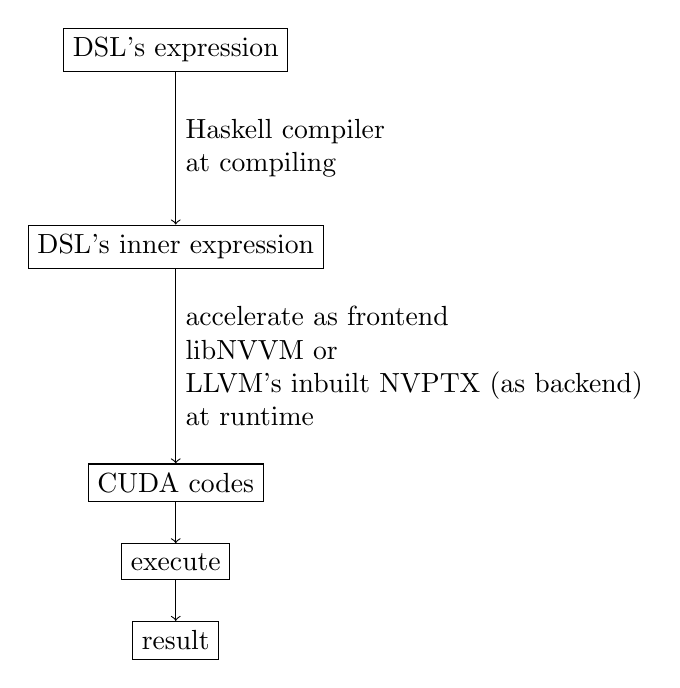
\begin{tikzpicture}[baseline=-.3em]
    \path
        (0,0)    node [draw,rectangle]  (exp) {DSL's expression}
     ++ (0,-2.5)   node [draw,rectangle]  (inner) {DSL's inner expression}
     ++ (0,-3)   node [draw,rectangle]  (cuda) {CUDA codes}
     ++ (0,-1)   node [draw,rectangle]  (exe){execute}
     ++ (0,-1)   node [draw,rectangle]  (rt){result}
     ;
    \draw [->] (exp)   -- node [right,pos=.5]{\vbox{\hbox{Haskell compiler}\hbox{at compiling}}}(inner);
    \draw [->] (inner) -- node [right,pos=.5]{\vbox{\hbox{accelerate as frontend}\hbox{libNVVM or } \hbox{LLVM's inbuilt NVPTX (as backend)}\hbox{at runtime}}}(cuda);
    \draw [->] (cuda) -- (exe);
    \draw [->] (exe) -- (rt);
    \end{tikzpicture}
    \caption{The workflow about how codes are executed}
    \label{fig:code:workflow}
\end{figure}

Firstly ,we just write the expressions of accelerate's DSL, in Haskell.
When using GHC or other Haskell compiler to compile those codes, the expression will be transform to
the DSL's inner expression. Then the something like JIT in accelerate will convert to the inner
expressions to the backend-specific codes via accelerate's frontend and a specific backend,
such as libNVVM, or LLVM's inbuilt NVPTX. After the codes in CUDA generated,
the codes will be translate into GPU, and after computing completed,
the results will be return back to program.

The program was tested with a serial $640 \times 640$ images, the details will be talk about at the section \ref{sec:test}. At this part, what is cared about is performance.

The figure \ref{fig:final-thread-legend} is the legend of those images generated by Haskell's event log
analysis tool \href{http://www.haskell.org/haskellwiki/ThreadScope}{Thread Scope}.
\begin{figure}
\centering
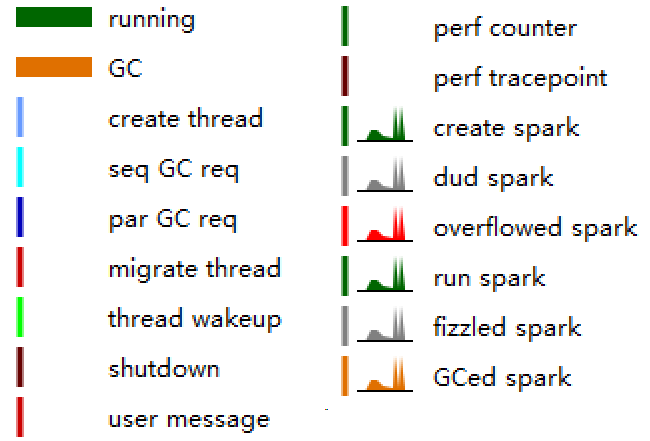
\includegraphics{final-thread-legend}
\caption{The legend of the images about the performance.}
\label{fig:final-thread-legend}
\end{figure}

For the test 1, the figure \ref{fig:fin-test1.bh} is thread performance of the test 1.

\begin{figure}
    \centering
    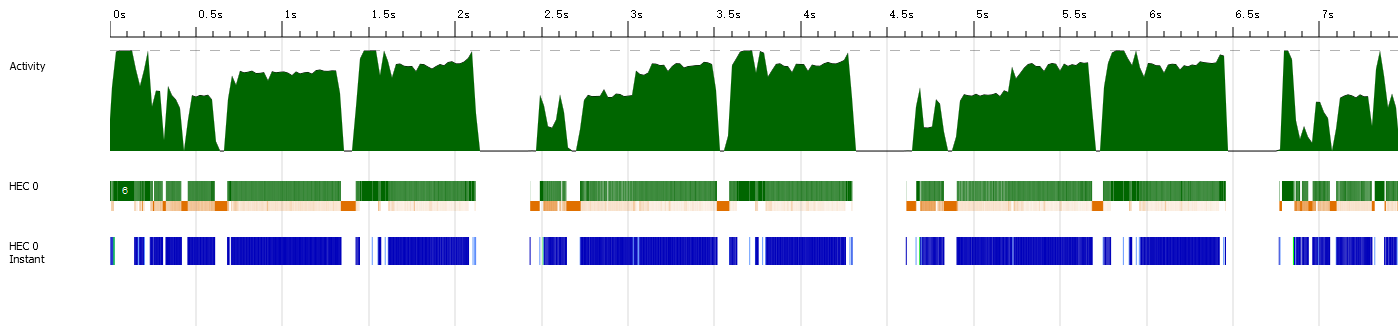
\includegraphics[width=1\linewidth]{fin-test1.bh.png}
    \caption{The thread performance of converting from BMP to Hpeg, in test1.}
    \label{fig:fin-test1.bh}
\end{figure}

From the beginning to the ending, the lifetime of the program is about 7.8s.
The large blank on the time line in the figure, is about waiting GPU to return the result.
The code generation of the libNVVM or LLVM's inbuilt NVPTX occupied the most resources of the CPU
to generate codes.
The figure \ref{fig:fin-test1.bh-detail} is the detail of the figure \ref{fig:fin-test1.bh}.

\begin{figure}
\centering
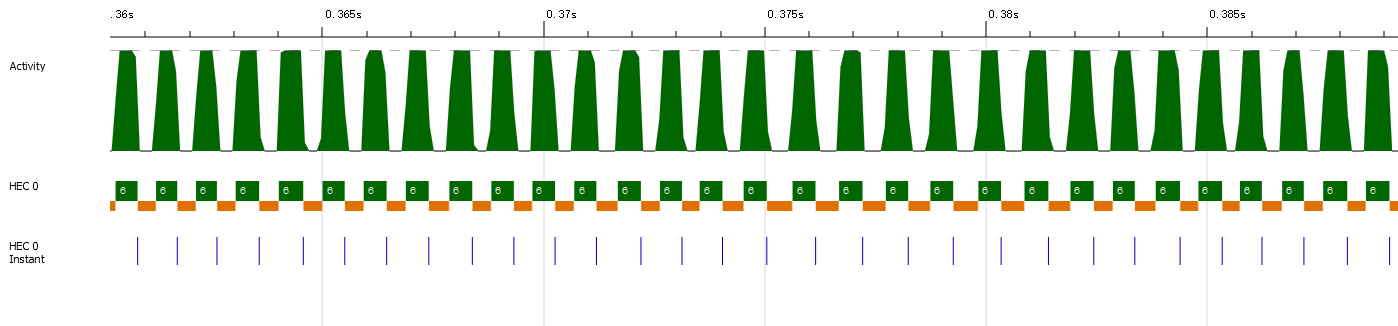
\includegraphics[width=1\linewidth]{fin-test1.bh-detail1.png}
\caption{The detail of figure \ref{fig:fin-test1.bh}.}
\label{fig:fin-test1.bh-detail}
\end{figure}

From the figure \ref{fig:fin-test1.bh} the main bottleneck of the program is on the CPU.
It take much more time on the generating than computing on GPU%
\footnote{The detail of the hareware where I test the program will be displayed on the section \ref{sec:test}}.

According to ThreadScope, the total time of the program is 7.45s, and the mutator time is 5.59s.
Meanwhile, it take 1.86s for garbage collection. The maximum size of heap is 141.0 MiB,
while GC totally collect about 2.9 GiB data, and it's rate of allocation is 538.7 MiB/s.
For just encoding the image, these may be horrible, but all this codes were written without optimization.

\subsubsection{Detail of DCT}
\label{sec:hpeg:performance:detail}

One of task in the Hpeg is transforming the matrix via DCT. Beacuse the nest-parallel is available,
when transforming a 2D matrix $A_{m \times n}$, the first thing to do is extending the
$A_{m \times n}$ to a 4D matrix $\widetilde{A}^{(i)}_{m \times n \times 8 \times 8}$. 
And there are more than one matrix like that needed. These matrices will be added together to
a single 4D matrix $\widetilde{A}_{m \times n \times 8 \times 8}$.
Final operation of the 4D matrix is folding it with ``plus``, and it will be a normal 2D matrix.

The complexities of both of time and space are $O(mn)$.
The samples of the tests are $640 \times 640$ images.
So it is not too slow, encoding such a image in few seconds, when the program without optimization.

\subsubsection{Ratio of Compression}
\label{sec:hpeg:performance:ratio}

The size of samples is 1228938 bytes, and all of the samples is in the form of Windows BMP with RGB.
The table \ref{tab:compression:size} show the sizes of the Hpeg files encoded from samples.
The best, or say minimum one is the sample No.1(figure \ref{fig:test:1}), 
which is full of a single color. Meanwhile the worst, or the maximum one is the sample
No.7(figure \ref{fig:test:7}), which is ``full'' of rainbows, but its ratio of compression
is still smaller than about $25\%$.

\begin{table}
    \centering
    \caption{The sizes of Hpeg files encoded from samples.}
    \begin{tabular}{|c|r|}
        \hline Sample No. & Size(bytes) \\
        \hline 1  &    1980 \\
        \hline 2  &  127772 \\
        \hline 3  &  126608 \\
        \hline 4  &  128188 \\
        \hline 5  &  145832 \\
        \hline 6  &  119592 \\
        \hline 7  &  306192 \\
        \hline 8  &  214108 \\
        \hline 9  &  128748 \\
        \hline 10 &  104540 \\
        \hline 
    \end{tabular} 
    \label{tab:compression:size}
\end{table}

\subsubsection{For Decoding}
\label{sec:hpeg:performance:decode}

The aboves are about the encoding, so in this part the topic is about decoding.
However, it is hard to find out the differences between the encoding and decoding,
for one is just the inverse of other one.

Using the test 1 as the example, the process of decoding is slower than the encoding.
Some one just might think that is a joke because Hpeg belong to some kinds of lossy compression,
and whatever the kind of Hpeg belong to, the decoding should be faster than encoding,
or just not slower than. But take it easy. For the example, it just slower about half second,
and there is not any optimization of the program. The figure \ref{fig:fin-test1} is the thread
performance of coverting from Hpeg to BMP.

\begin{figure}
\centering
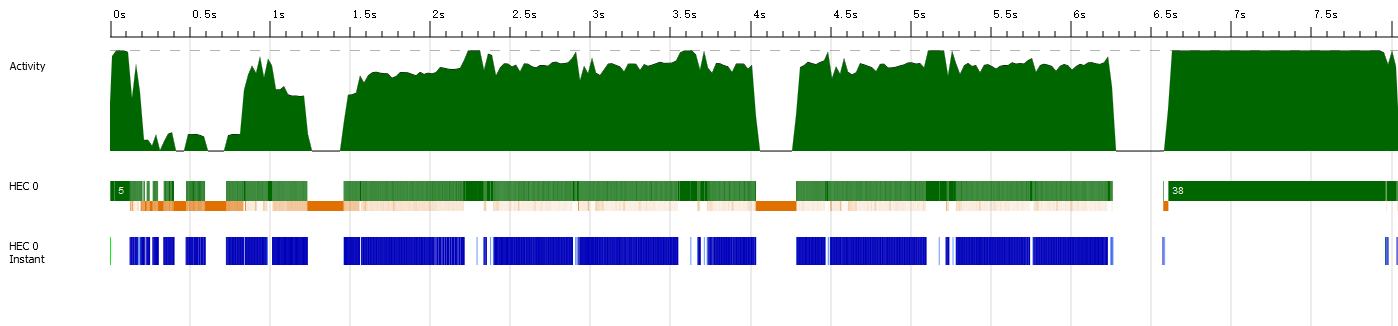
\includegraphics[width=1\linewidth]{fin-test1.hb.png}
\caption{The thread performance of coverting from Hpeg to BMP.}
\label{fig:fin-test1}
\end{figure}

Its total time of running is 8.04s, and mutator time is 6.19s. Meanwhile, the time spend on garbage collection is about 1.85s. The maximum size of the heap is  371.0 MiB,
and at the same time, it totally allocated 2.8 GiB data, whose rate is 462.4 MiB/s.

%% test
\section{Test}
\label{sec:test}

In this section, the influence of noises will be the hero, and at the same time,
the test of the program is going to be heroine.
 
\subsection{Environment}
\label{sec:test:environment}

Before the main part of this section, there are two things to do: let me have a drink,
and show the details of where I test the program.

The tests were done on a pool dusty computer. The CPU of it is a AMD Athlon(tm) II X4 641 Quad-Core Processor, ans it has 8GB RAM.
More, there is a Nvidia's GeForce GTX 960, which has 2GB global memory, with 128-bit width memory
bus, and 1024 CUDA cores in 8 multiprocessors.

That's hardware, and the following is software. 

Its operating system is kubuntu 17.04 with Linux's 4.10 kernel. In the computer,
the CUDA driver version 8.0 is installed. Meanwhile, the version of the Haskell's compiler is 
8.0.2. 

\subsection{Basic Test \& Result}

Before analyzing the influence of noises, let talk about the heroine -- test itself.
The program tested with 10 $640 \times 640$ images, in the form of Windows BMP.
And all of the test samples are in figure \ref{fig:test}.

\begin{figure}
\centering
\subfigure[Sample No.1]{
    \label{fig:test:1}
    
\includegraphics[width=1.0in]{hpeg-test/test1}}
\subfigure[Sample No.]{
    \label{fig:test:2}
    
\includegraphics[width=1.0in]{hpeg-test/test2}}
\subfigure[Sample No.3]{
    \label{fig:test:3}
    
\includegraphics[width=1.0in]{hpeg-test/test3}}
\subfigure[Sample No.4]{
    \label{fig:test:4}
    
\includegraphics[width=1.0in]{hpeg-test/test4}}

\subfigure[Sample No.5]{
    \label{fig:test:5}
    
\includegraphics[width=1.0in]{hpeg-test/test5}}
\subfigure[Sample No.6]{
    \label{fig:test:6}
    
\includegraphics[width=1.0in]{hpeg-test/test6}}
\subfigure[Sample No.7]{
    \label{fig:test:7}
    
\includegraphics[width=1.0in]{hpeg-test/test7}}
\subfigure[Sample No.8]{
    \label{fig:test:8}
    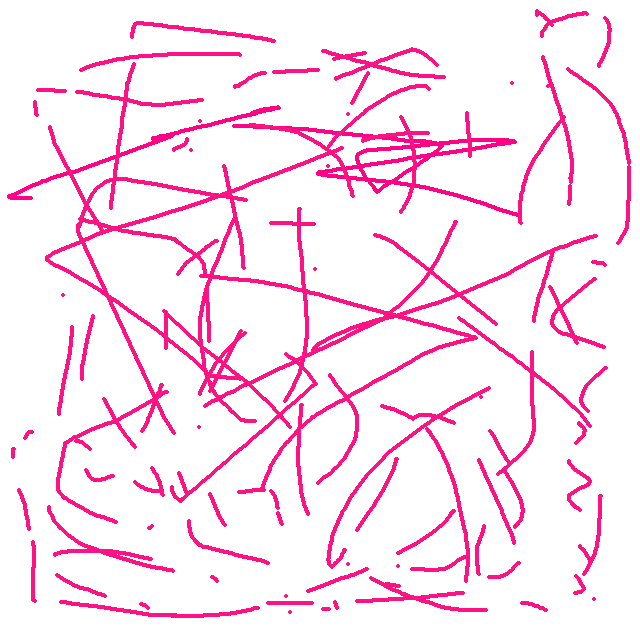
\includegraphics[width=1.0in]{hpeg-test/test8}}

\subfigure[Sample No.9]{
    \label{fig:test:9}
    
\includegraphics[width=1.0in]{hpeg-test/test9}}
\subfigure[Sample No.10]{
    \label{fig:test:10}
    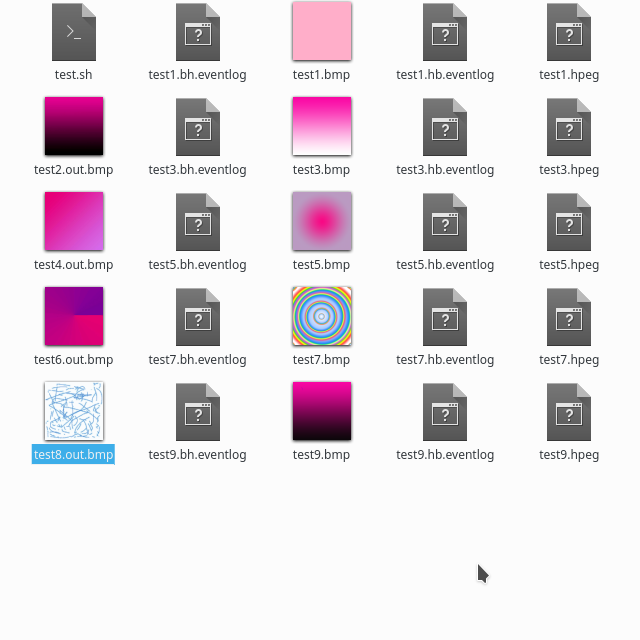
\includegraphics[width=1.0in]{hpeg-test/test10}}
\caption{Test samples}
\label{fig:test}
\end{figure}

The sample No.1 is a image with a single color. The samples No.2 ~ No.6, and No.9 are the images with
color changed smoothly. The sample No.7 is the image full of rainbow, whose color changed
both smoothly in the detail but sharply in the range of color. The sample No.8 is
the image to test the noise. The sample No.10 is the screen shot of the computer.

All these images are created in the Photoshop and saved in the form of Windows BMP.

\subsection{Results of tests}
\label{sec:test:result}

So the result of these tests are all in the figure \ref{fig:result}.

\begin{figure}
    \centering
    \subfigure[Result No.1]{
        \label{fig:result:1}
        
\includegraphics[width=1.0in]{hpeg-test/test1.out.png}}
    \subfigure[Result No.2]{
        \label{fig:result:2}
        
\includegraphics[width=1.0in]{hpeg-test/test2.out.png}}
    \subfigure[Result No.3]{
        \label{fig:result:3}
        
\includegraphics[width=1.0in]{hpeg-test/test3.out.png}}    
    \subfigure[Result No.4]{
        \label{fig:result:4}
        
\includegraphics[width=1.0in]{hpeg-test/test4.out.png}}
    
    \subfigure[Result No.5]{
        \label{fig:result:5}        
        
\includegraphics[width=1.0in]{hpeg-test/test5.out.png}}
    \subfigure[Result No.6]{
        \label{fig:result:6}
        
\includegraphics[width=1.0in]{hpeg-test/test6.out.png}}    
    \subfigure[Result No.7]{
        \label{fig:result:7}
        
\includegraphics[width=1.0in]{hpeg-test/test7.out.png}}
    \subfigure[Result No.8]{
        \label{fig:result:8}
        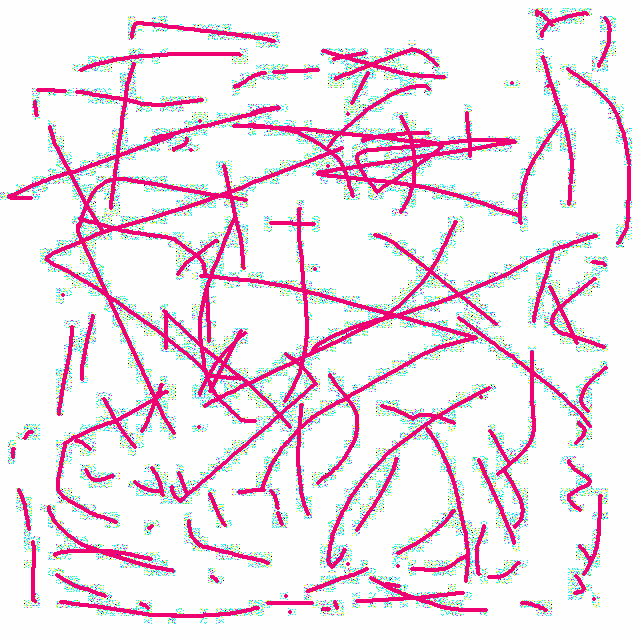
\includegraphics[width=1.0in]{hpeg-test/test8.out.png}}
    
    \subfigure[Result No.9]{
        \label{fig:result:9}
        
\includegraphics[width=1.0in]{hpeg-test/test9.out.png}}    
    \subfigure[Result No.10]{
        \label{fig:result:10}
        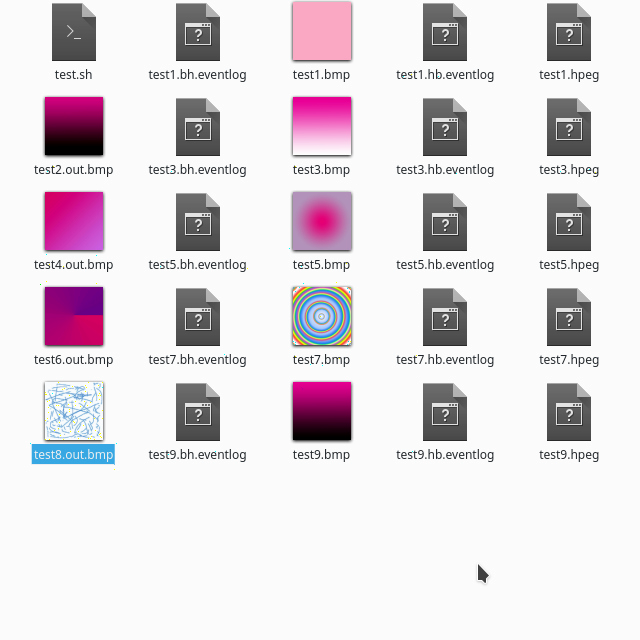
\includegraphics[width=1.0in]{hpeg-test/test10.out.png}}    
    \caption{Test result}
    \label{fig:result}
\end{figure}

If you are read a printed copy of this report, the detail of the detail of result will miss.
If you are read the copy in the PDF form, you can try to zoom in on the details of each figure,
and you can the sharp errors in the figures.


\subsection{Hero -- Analysis of Noises}
\label{sec:test:analysis}

The most common definition of the noise might be ``unexpcepted disturbances in the source of signal 
or in the process of translation''. In other word, the unexpected things, which you don't want,
is the noise.

So in figure \ref{fig:test:6}, figure \ref{fig:test:7} and figure \ref{fig:test:8},
 the sharp changed color, or say turn-round-like color changing can be regarded as the noise.
 
In figure \ref{fig:result:6}(figure \ref{fig:ana:1} show the details), the difference between two color
is mainly in luminance. Meanwhile such ``noise'' hardly has the influence on the image.

\begin{figure}
\centering

\includegraphics[width=0.7\linewidth]{hpeg-test/ana1}
\caption{The details of the figure \ref{fig:result:6}}
\label{fig:ana:1}
\end{figure}

In figure \ref{fig:result:7}(figure \ref{fig:ana:2:1} show the details), there are some ``thorns'' at\
the four corner of the image. These ``thorns'' are here, because of the ``noise'' of the write background.
So the noise in the white background make the ``thorns'' in the image, and the figure \ref{fig:result:8}(figure \ref{fig:ana:2:2} show the details) is another example.

\begin{figure}
    \centering 
    \subfigure[Detail of figure \ref{fig:result:7}]{
        \label{fig:ana:2:1}
        
\includegraphics[width=1.0in]{hpeg-test/ana2}} 
    \hspace{0.5in}
    \subfigure[Detail of figure \ref{fig:result:8}]{
        \label{fig:ana:2:2}
        
\includegraphics[width=1.0in]{hpeg-test/ana3}} 
    \caption{The details of results}
    \label{fig:ana:2}
\end{figure}

However, the ``thorns'' disappear in the figure \ref{fig:result:10}(figure \ref{fig:ana:3} show the detail).
The between the white background and the icons, it is difficult to find the ``thorn''.

\begin{figure}
\centering

\includegraphics[width=0.67\linewidth]{hpeg-test/ana4}
\caption{The detail of figure \ref{fig:result:10}}
\label{fig:ana:3}
\end{figure}

So that means the ``thorn'' will appear when some specific-color noise in the source.
Meanwhile the gray might be a good color to insulate those colors which might cause the ``thorn''.

\paragraph{Conclusion}
The noise itself might influence the surrounding image, but just in the $8 \times 8$ area because of 
the DCT. A noise, which is red thorn with white background, will cause the other thorn,
but if the noise is gray, that might not happen.  

%% improvement
\section{Improvement}
\label{sec:improvement}

To be honest, the program tested is already improved one. The thorn both of noise and image itself,
appear because the lost of the information in the color. When quantizing, if the value rounded down
to integer, there will be so many thorns in the image. Meanwhile, if the information of the color
reserved too much, the size of the image will be larger. So the program reserved additional 5 bits
of the color's value.

Another way to improve it quality is change another color space to store the image, which should suit
the DCT.

\end{document}